\providecommand{\main}{..}
\documentclass[\main/main.tex]{subfiles}

\begin{document}
\lesson{14}{12/11/20}

\subsection{Reaction-diffusion model}
Let's highlight the connection of DP with a very used and popular model, called \textit{reaction-diffusion}, whose name is due to the fact that it combines diffusion (the fact that particles in the model are moving around diffusing) and reaction (the number of entities in the model can change).

This kind of model is used to describe the combination of chemical reactions with the diffusion of the chemical species involved in the reaction.

In the context of DP we can show some examples in Figure \ref{fig:rd}: in the first sketch we can show two examples of diffusion: the active site is moving either to the left or to the right (like a unbiased random walk in $2d$). Another possibility is the case of a 'death' process in which all the active sites are disappearing all together or one more active site can appear. like in the 'offspring' generation. 
Another typical case is the 'coalescence' in which two active sites becomes just one at $t+1$.

\begin{figure}[ht]
    \centering
    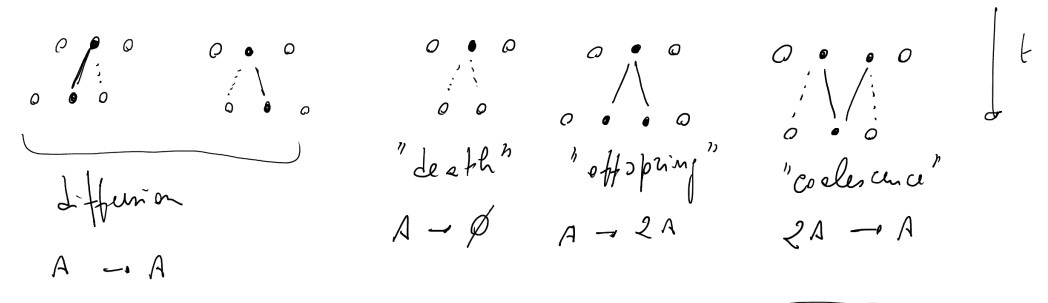
\includegraphics[width=\linewidth]{Lectures/Images/sas.jpg}
    \caption{Examples of directed percolation in different contexts. $A$ stands for '\#active site'.}
    \label{fig:rd}
\end{figure}

We can realize from Figure \ref{fig:rd} that in order to define those events (which are not really stochastic update rules) we had to put together different nearby sites to properly describe those events but the point is that DP can be seen at a very simple level as a reaction of a model which combines reactive and diffusive events.

\section{Generalization of DP: The Domany–Kinzel Model of Cellular Automata}

Many basic models of non-equilibrium phase transitions can be formulated as dynamical processes of interacting particles moving on a lattice. When a lattice site can be either occupied by a single particle or empty (exclusion process) and the evolution rule is local, synchronous, and Markovian, the model at hand is just a cellular automaton (CA).

In other words cellular automata (CA) is a binary model based on a lattice, so the sites of the lattice can be either \textit{active} or \textit{inactive} (\textbf{exclusion process}: there cannot be double occupancy of the sites).
CA is also characterized by 
\begin{itemize}
    \item \textit{Local evolution rules}: the evolution rules depend only on neighbouring sites;
    \item \textit{Synchronicity}: sites can be updated in parallel (DP is an example);
    \item \textit{Markovianicity}: what happens at $t+1$ depends only on the history at the previous time $t$.
\end{itemize}

In addition CA can be either \textit{deterministic} (with deterministic evolution update rules) or \textit{stochastic} (stochastic update rules): DP and the DK model are examples of stochastic cellular automata.

The stochastic update rules in the Domany-Kinzel model are the ones presented in Figure \ref{fig:stoch_rules}:

\begin{figure}[ht]
    \centering
    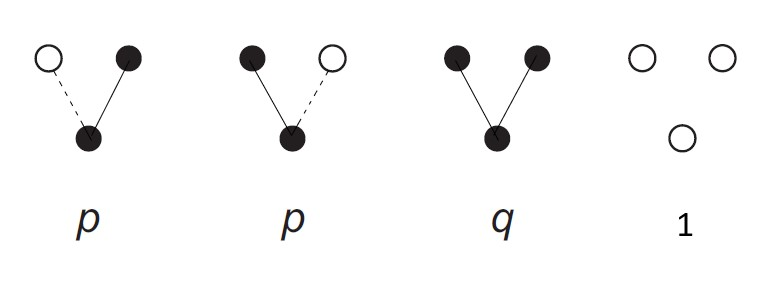
\includegraphics[width=0.8\linewidth]{Lectures/Images/stoch_rules.jpg}
    \caption{Probabilistic evolution rules. The cases in which the final site is inactive can be recovered through normalization.}
    \label{fig:stoch_rules}
\end{figure}

The third event of Figure \ref{fig:stoch_rules} is associated to a probability $q$, so in the DK model we are dealing with two different parameters, $p,q$: $p$ is the probability of diffusive event, while $q$ is the probability of the coalescence event. \\

The phase diagram in the $(p,q)$ plane is the one represented in Figure \ref{fig:phase}: we can see a transition line (the solid one) such that on the right of it we have the active phase while on the left the inactive phase.

The main point is that we have a critical line $p_c(q)$ (for any value of $q$ we have a percolation threshold as a function of $q$) and for all $q$ strictly less than unity ($0\leq q <1$) we are in the same universality class of DP and only for $q=1$ the universality class is changed and we move to another kind of non-equilibrium phase transitions called \textit{compact directed percolation (CDP)}.

For $q=1$ the corresponding percolation threshold is $1/2$ and we will discuss later why is that true. \\

We can now choose different examples of directed percolation in order to see how they are realized in the context of the DK model:\\

\textbf{Bond directed percolation} \\
We already saw that the event called 'coalescence', to which a  probability $q$ is associated in the DK model, for BDP $q$ is just related to the following function:
\begin{equation}
    q=p(2-p)
\end{equation}
which is a parabola in the $(q,p)$ plane, as represented in Figure \ref{fig:phase}. \\

\textbf{Site directed percolation} \\
Looking closer to the coalescence event in site percolation $p$ is the probability of a site being active, so the probability that the site below two active sites is active is just $p$: we don't have to look to bond activation but only to site activation, so $q=p$, represented in Figure \ref{fig:phase} as the diagonal of the square. \\

Bond and site percolation share the same universality class but the percolation threshold is different.

\begin{figure}[ht]
    \centering
    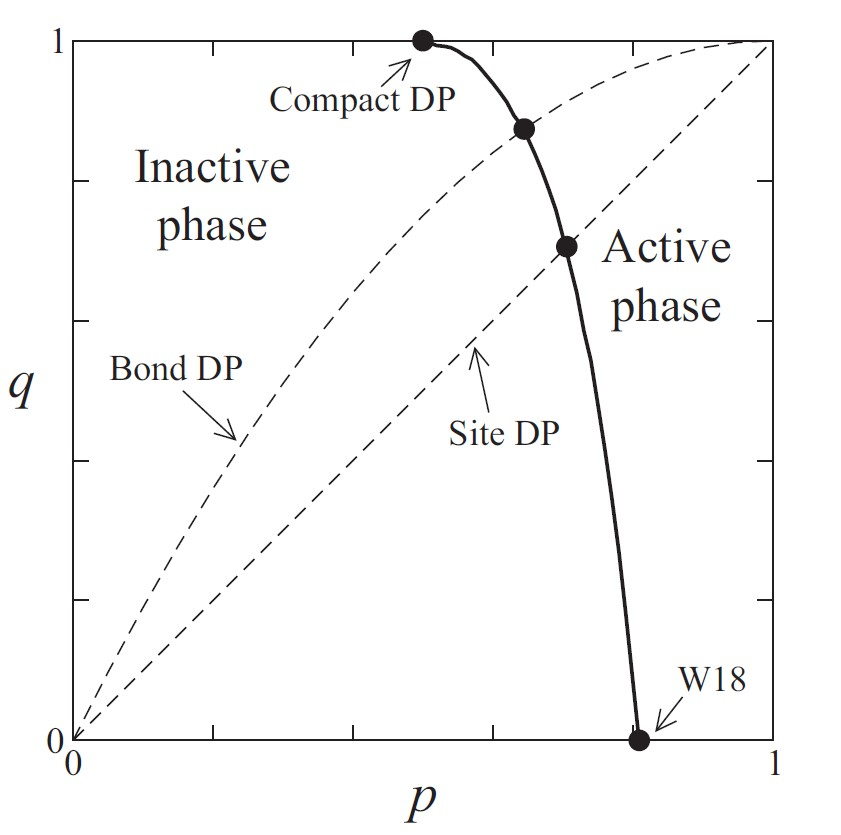
\includegraphics[width=0.5\linewidth]{Lectures/Images/phase_diag.jpg}
    \caption{Phase diagram of the DK model. The thick solid line is the curve $p_c(q)$, separating the absorbing (inactive) phase from
the active one. The dashed lines correspond to the bond DP $(q = p(2 - p))$ and to the site DP percolation $(q = p)$.}
    \label{fig:phase}
\end{figure}

Another example is $q=0$: in this case the site below two active sites is always inactive and essentially there is no coalescence, called $\mathbf{W18}$ because it's a stochastic version of an update rule listed as Wolfram classification.

The last peculiar example is at $q=1$: this is a different universality class, called \textit{compact DP}, with $p_c=1/2$ due to a 'symmetry' between active and inactive sites: when $q=1$ we can also see the situation in which all the sites are active becomes an absorbing phase in the system, having two possible absorbing states\footnote{This is why the universality class changes for $q=1$.} in the system (all sites empty and they keep being empty or all sites active and they keep staying active because $q=1$). \\

It is also interesting how the percolating clusters look like at the percolation transition: in Figure \ref{fig:clusters} we see, as a function of $p$, the fractal nature of the percolating clusters right at the transition.

The quantity on the $y$ axis is the average size of active spots which are stretches of active sites without holes in between: in a given time we can have different stretches and we can take the average of their size.

The higher is $p$ the clusters presents several holes, which corresponds to low values of the $\mean{S_{act}}$ parameter. If we increase $q$ then the corresponding percolation threshold is increasing and we can see e.g. BDP the holes are decreasing and $\mean{S_{act}}$ increasing.

In the limit of $q\to 1$ and therefore the percolation threshold going to $1/2$ what happens is that holes disappear and essentially this is why the CPD are called in this way: the cluster are not fractal objects anymore.

\begin{figure}[ht]
    \centering
    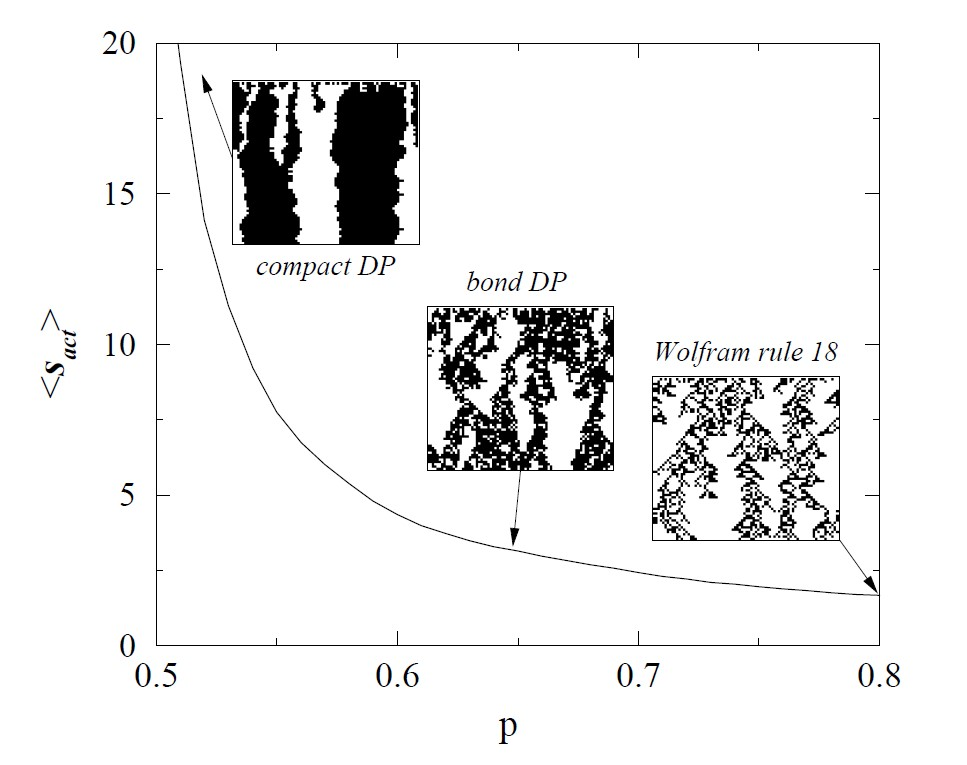
\includegraphics[width=0.7\linewidth]{Lectures/Images/clusters.jpg}
    \caption{Numerical estimates for the average size of active spots $\mean{S_{act}}$ in the Domany-Kinzel model measured along the phase transition line. The insets show typical clusters for three special cases discussed
in the text.}
    \label{fig:clusters}
\end{figure}

Figure \ref{fig:as} is reported in order to clarify what 'active spots' means: to the right wee ave two different active spots, one of size 2 and one of size 3

\begin{figure}[ht]
    \centering
    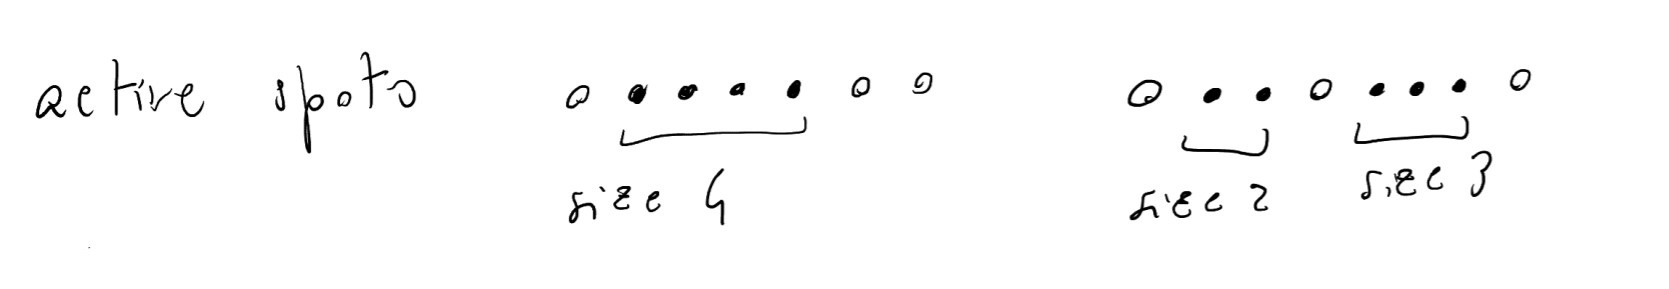
\includegraphics[width=0.9\linewidth]{Lectures/Images/as.jpg}
    \caption{Active spots' graphical interpretation.}
    \label{fig:as}
\end{figure}

\section{The Phase Transition in DP-like Systems}
\subsection{Order Parameters, Correlation lengths and Critical Exponents}

We define as \textit{control parameter} the probability $p$ (comparable to )

The DP class of non-equilibrium phase transitions to one single absorbing state is characterized by typical scaling properties at the transition point that are widely reminiscent of critical phenomena in the equilibrium case. For instance, the ferromagnetic transition in the Ising model (which will be used as a comparison) is found to occur at a critical temperature $T_{\mathrm{c}},$ where the magnetization vanishes as $M \sim\left(T_{\mathrm{c}}-T\right)^{\beta} .$ The temperature $T$ and the magnetization $M$ are the control and the order parameter of this phase transition, respectively. The divergence of the correlation length as $\xi \sim\left|T-T_{\mathrm{c}}\right|^{-\nu}$ implies that very close to $T_{\mathrm{c}}$ there is no typical macroscopic length scale; i.e., the physical system is invariant under scale transformations. From the discussion in the previous section, one can easily infer that in the DP class the natural control parameter, analogous to the temperature $T$ in the equilibrium case, is some probability $p,$ e.g., the probability of an open channel in bond DP/site activation, the parameter $p(q)$ in the DK model or the ratio $(\lambda / r)$ in the contact process. As in equilibrium phenomena, the critical value of the control parameter\footnote{The value of the control parameter is not universal: the critical value of the control parameter is non-universal, in a similar way of what happens in equilibrium phase transitions.}, $p_{c}$, is a model-dependent quantity.

As for the order parameter, in DP-like systems there are two possible ways to define it: (i) we can count the active sites and evaluate asymptotically in time their number (or their density), which must vanish in the inactive phase or (ii) we can evaluate the probability of not yet having reached the absorbing phase at time $t$ (and, again, taking the limit $t \rightarrow \infty$ ). More precisely, the first choice depends on the initial conditions, which may be characterized by a vanishing or a finite density of active sites. In the former case (think of the limiting case of one single active site at $t=0$ ) the morphology does not scale with the size of the system and we must simply count the number of active sites,
$$
N(t)=\left\langle\sum_{i} s_{i}(t)\right\rangle
$$
where the ensemble average $\langle\bullet\rangle$ is performed over many realizations of the stochastic evolution. For homogeneous initial conditions, instead, we should use the density of active sites\footnote{The density of active sites can actually be evaluated even for a single, initial active site if we normalize $N(t)$ with respect to $t,$ which is the maximal possible number of active sites at time $t,$ starting from a single active site.}
$$
\rho(t)=\frac{1}{L} \sum_{i}\left\langle s_{i}(t)\right\rangle=\frac{N(t)}{L}
$$
where $L$ is the total number of sites. The second choice for the order parameter is the survival probability for a trajectory whose initial state has one active site only, $s_{i}(0)=\delta_{i, k}$. It can be formally defined as
$$
P(t)=\left\langle 1-\prod_{i}\left(1-s_{i}(t)\right)\right\rangle
$$

where $P(t)$ is the ensemble average of an observable that is equal to 1 until an active site
is present, while it vanishes only when the system evolves into the fully inactive absorbing
state. In other words, $P(t)$ is the fraction of the ensemble of stochastic evolutions that at
time t have not yet reached the absorbing state.

Comparing DP with Ising model what we get is:

\begin{itemize}
    \item \textit{Control parameter}: the control parameter is the bond/site activation $p$\\
    \[T \longleftrightarrow p\,\, \text{or}\,\, (p,q) \,\, \text{in DK}\,\, \]
    \item \textit{Order parameter}: in the Ising model the magnetization density is used (average spin value): In the context of DP we can have different possible order parameters and it may depend for example on the kind of initial conditions that one is using: for example for one initially active site we can use (\ref{eq:n}) while for homogeneous initial conditions (fixed fraction of initially active sites) we can use $\rho(t):=N(t)/L$
    \begin{numcases}{m := \frac{\mean{\sum_i S_i}}{L} \longleftrightarrow}
    N(t):=\mean{\sum_is_i(t)} &  1 IAS\\
    \rho(t):=N(t)/L &  F.F. of IAS \\
    P(t):=\mean{\hlc{yellow}{1-\prod_{i=1}^L(1-s_i(t))}} & S.P.
    \label{eq:hehe}
    \end{numcases}
    It is important to state that the first average us over different realizations of a stochastic process, while the Ising one is just the thermodynamic ensemble average.
    
    The last possible order parameter for a trajectory with one initially active state is called \textit{survival probability}, defined as the average over different realizations of (\ref{eq:hehe}). The factors in the product are either 0 when the site is active or 1 when the site is inactive so the whole product is 1 $\iff$ all sites are empty or zero otherwise: this means that the yellow quantity is 0 for all empty/inactive sites or 1 for any other state with at least one active site.
    Taking then the average over all realizations of this quantity the survival probability is the fraction of survived trajectories, so $0\leq P(t)\leq 1$ and 0 means that all trajectories at time $t$ eventually end up in the absorbing phase, where all sites are empty. On the other hand $P(t)=1$ means that all trajectories survived and none of the trajectories reached the absorbing phase;
\item \textit{Order with limits}: dealing with non-equilibrium phase transitions we also have time and we are interested in what is going on asymptotically at infinite time, therefore we have two limits: $t\to\infty$ and $L\to\infty$. The order in which these two limits are taken is very important: the correct order is first (for fixed time) taking the thermodynamic limit of infinite size system and then infinite time limit. This is the correct order to describe asymptotic behaviour in the thermodynamic limit.

Doing the way around what we get is the asymptotic behaviour for a finite system, no matter how big it is: to study the property of an infinite size system the right limit order is the latter one. \\

The three order parameters that we introduced are zero in the inactive phase and they're greater than zero in the active phase: in this sense they are good order parameters.

\item \textit{Critical exponents}: In the limit $t\to\infty$ - in analogy to equilibrium phase transitions - these order parameters can be associated to critical exponents as:

\begin{numcases}{m\sim(T_C-T)^\beta \longleftrightarrow}
\rho(\infty) \sim\left(p-p_{c}\right)^{\beta} &\\
P(\infty) \sim\left(p-p_{c}\right)^{\beta^{\prime}} &
\end{numcases}
where the behaviour of the order parameter is similar to the curve represented in Figure \ref{fig:fig} and the behaviour very close to the transition point is a power law and it defines the critical exponent $\beta$ (as the exponent used in equilibrium phase transitions).

These relations indicate that when approaching the critical point $p_{c}$ from the active phase, $p>p_{c},$ both order parameters vanish according to a power law. It is customary to associate the survival probability with the annihilation process and the density of active sites with the creation process, so $\rho(t)$ and $P(t)$ are sometimes referred to as creation and annihilation order parameters, respectively.

It is not obvious to say a priori if $\beta$ and $\beta^{\prime}$ should be equal or not\footnote{A primary criterion seems to be related to the number of absorbing states, as shown by the DK model.}: in general $\beta\neq\beta'$ and for $q=1$ in the case of the DK model with Compact DP $\beta\neq\beta'$ whereas for $q<1$ the DK model (DP) belongs to the bond DP universality class, has only one absorbing state and $\beta=\beta^{\prime} \simeq 0.276$ in $1d$.

Let's now justify the fact that in DP $\beta=\beta'$ in the special case of Bond DP: we can actually show that the two order parameters are indeed the same quantity
\begin{equation}
    P(t)=\rho(t)
\end{equation}

because of time reversal symmetry, which holds only in the BDP case.
\end{itemize}

Let's now compute the survival probability $P(t)$: in Figure \ref{fig:sp} we are drawing a trajectory where some branches die and some other survive until time $t$. Let's now take the bottom row and consider the time reversal (we have a full time reversal symmetry only in the case of BDP also because of the fact that we chose this tilted square lattice): let's consider all sites initially active and then let's consider all trajectories after reversing time.
   
\begin{figure}[ht]
    \centering
    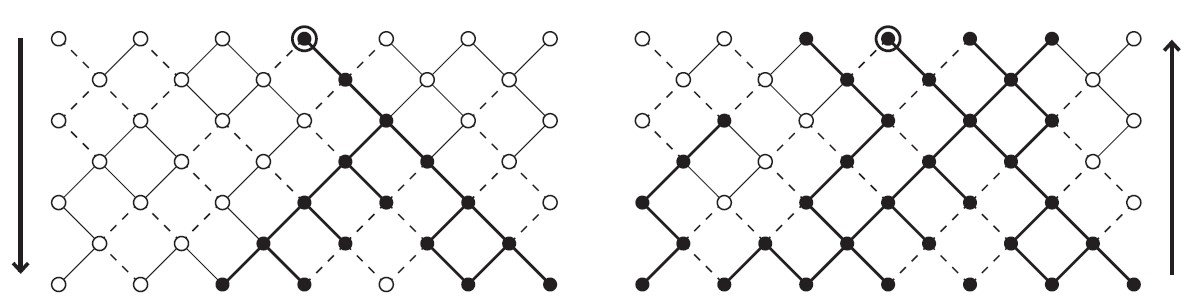
\includegraphics[width=0.8\linewidth]{Lectures/Images/sp.jpg}
    \caption{Left: Directed percolation process starting from a single active site. Right: Time-reversed process of the left one,
starting from a fully active state. If there is one directed path from top to bottom (left), there must be a directed path
from bottom to top (right).}
    \label{fig:sp}
\end{figure}

The point is that if we consider the fraction of active sites on top of the right of Figure \ref{fig:sp} having started with all initially active sites on bottom is equal to the fraction of survived trajectories from top, because if we can go from bottom to the top and we see something acting to the top this means (due to time reversal symmetry) that we can start from that site active in the top and then reach back to the bottom.

When we say 'fraction of survived trajectories' it is a fraction in which we average over the different possible location/positions of the initially active sites, but in the definition of S.P. we need to average over different realizations of the system.

It turns out that those two kinds of averages (average over different initial conditions and average over different realizations of a stochastic process) provide the same result under the so called \textit{self-averaging condition}: in general dealing with heterogeneous systems or with stochastic processes one has to perform an average over different realizations of the system and in this case over different possible trajectories or in a spin-glass over different samples of material for example.

The point is that, if a quantity is self-averaging what happens we can average over different subsets of the system: formally self-averaging holds only in the thermodynamic limit and instead of choosing always the same site as initially active and then to run the stochastic process at different times we can choose the same site as initially active and then try a trajectory various times (average over different realizations) we can average over different positions of the initially active site and if the system is big enough the sampling of different trajectories is the same as sampling different realizations starting from the same point. 

The only rigorous proof that $\beta=\beta'$ is for BDP but numerically it can hold also for other examples of DP because $P(t)\overset{t>>1}{\sim}\rho(t)$. \\

\textit{From the book}: 
The equivalence between the exponents $\beta$ and $\beta^{\prime}$ in DP is a consequence of a special symmetry of this model, which amounts to a sort of time-reversal symmetry. A heuristic explanation can be given in the case of bond DP, considering a configuration of open and closed bonds as the one shown in Figure \ref{fig:sp}. The quantity $P(t)$ is evaluated in direct time (left panel) activating a single site and determining if there is a directed path through active bonds, leading to the opposite (bottom) side. If we are in the thermodynamic limit, the average over disorder realizations can be replaced, using self-averaging, by an average over the starting site, so $P(t)$ is just the fraction of initial sites that are connected to the opposite side. Now we revert the time arrow, as shown in the right panel of the same figure: we start from all active sites and evaluate the density of active sites at time $t, \rho(t)$ It is clear that a "top" site is now active if and only if there is a directed path connecting it to the bottom side, which is exactly the condition because, in direct time, it contributes to $P(t) .$ In conclusion, if we average over disorder or we take the limit $L \rightarrow \infty,$ we expect that
$$
P(t)=\rho(t)
$$
Accordingly, in the active phase both order parameters $P(\infty)$ and $\rho(\infty)$ have to saturate to the same value and have to exhibit the same critical behavior at $p_{c} ;$ i.e., $\beta$ and $\beta^{\prime}$ have to be the same critical exponent. This equivalence holds also for other kinds of DP processes such as site DP or the contact process, although the same argument based on the exact time-reversal symmetry typical of bond DP does not apply. Nonetheless, there is numerical evidence that this symmetry still holds asymptotically, while $P(t)$ and $\rho(t)$ become proportional to each other in the long time limit and $\beta=\beta^{\prime}$.\\

Let's now discuss the \textit{correlation lenght}: the main feature that makes non-equilibrium critical phenomena different from equilibrium ones is the presence of independent spatial $\left(\xi_{\perp}\right)$ and time $\left(\xi_{\|}\right)$ correlation lengths, where the $\perp$ and $\|$ symbols refer to the time arrow. These quantities are associated with the asymptotic behavior of the space and (positive) time correlation functions

\begin{equation}
c_{|i-j|}:=\left\langle\lim _{t \rightarrow \infty} \frac{1}{t} \sum_{\tau=0}^{t}\left(s_{i}(\tau)-\bar{s}\right)\left(s_{j}(\tau)-\bar{s}\right)\right\rangle \sim e^{-|i-j| / \xi_{\perp}} 
\label{eq:specialtC}
\end{equation}

\begin{equation}
 c(t)=\left\langle\lim _{L \rightarrow \infty} \frac{1}{L} \sum_{i=1}^{L}\left(s_{i}(0)-\bar{s}\right)\left(s_{i}(t)-\bar{s}\right)\right\rangle \sim e^{-t / \xi_\|} 
 \label{eq:specialxC}
\end{equation}


where $i,j$ are the position of two different sites (and they refer to spatial coordinates) and the average (over different realizations) value
$$
\bar{s}=\lim _{t \rightarrow \infty} \frac{1}{t} \sum_{\tau=0}^{t}\left\langle s_{i}(\tau)\right\rangle
$$
does not depend on the site index (the limit of infinite time is crucial).

\begin{figure}[ht]
    \centering
    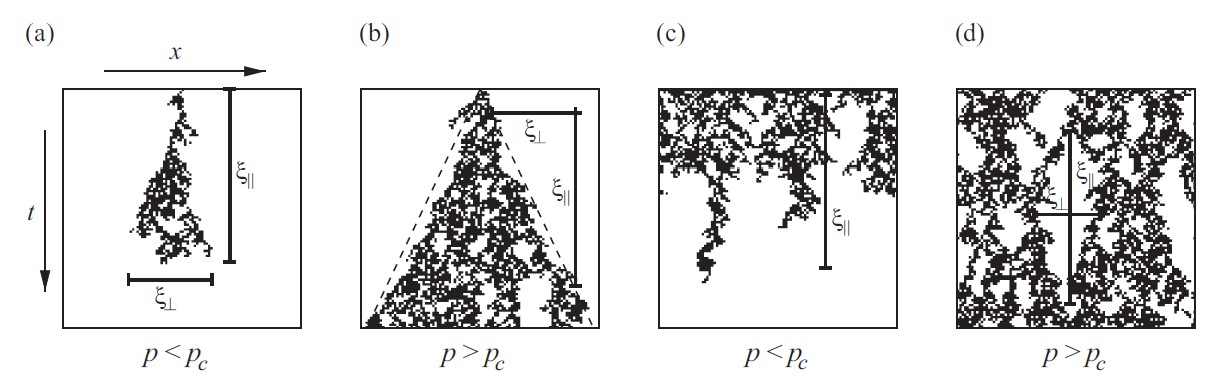
\includegraphics[width=\linewidth]{Lectures/dddddd.jpg}
    \caption{Pictorial description of the correlation lengths $\xi_{||}$ and $\xi_{\perp}$ in a DP process for different initial conditions, below and above criticality. The explanation for part labels (a)–(d) are discussed in the text.}
    \label{fig:interepretazione}
\end{figure}

The physical interpretation of the temporal and spatial correlation lenghts $\xi_{||}$ and $\xi_{\perp}$ is represented in Figure \ref{fig:interepretazione}. In the subcritical phase (a) $p<p_c$, $\xi_{\perp}$ is the typical size of a cluster and $\xi_{||}$ is the typical time of clusters before they disappear: in the inactive phase eventually all active sites disappear and so the correlation time is the typical survival time of the cluster.

On the other hand in the supercritical phase $p>p_c$ (b) $\xi_\perp$ is the typical size while $\xi_\|$ is the typical duration time of islands of empty sites within clusters: in phase (b) we have a spanning cluster going from top to bottom, as big as the system' size but we have holes in it (\textit{islands of empty sites}) that appear and disappear (it's a fluctuating phase).
In the supercritical phase one can see that the ratio $\xi_\perp/\xi_\|$ is related to the cone opening: if we start with one initially active site the cluster will grow and the opening of the cone is related to the previous ratio. \\

Of course when we are approaching the percolation threshold both the two correlation length diverges, so in this way we can define two more critical exponents: very close to $p_{c}$ both correlation lengths are found to diverge as

\begin{align}
\xi_{\perp} & \sim\left|p-p_{c}\right|^{-\nu_{\perp}} \\
\xi_{\|} & \sim\left|p-p_{c}\right|^{-\nu_{\|}}
\end{align}

for $p\to p_c$.
A very important quantity used in describing non-equilibrium phase-transitions is the \textit{dynamical exponent} $z$:
\begin{equation}
    z:=\frac{\nu_\|}{\nu\perp}
\end{equation}

From a practical point of view, the most efficient order parameter for determining the critical point of DP processes by numerical simulation is the average cluster mass which is found to grow algebraically at $p_c$ as

\begin{equation}
    N(t)\sim t^\theta \quad \text{for}\,\, p=p_c
\end{equation}

It can be shown\marginpar{Scaling laws}, also in out-of-equilibrium phase transitions, that one deals with \textbf{scaling laws} between different critical exponents :
\begin{equation}
    \theta=\frac{d\nu_\perp - \beta-\beta'}{\nu_\|}
    \label{eq:scaling}
\end{equation}
where $d$ is the spatial dimension. \\
Let's show that scaling theory can be used also for non-equilibrium phase transitions.

\subsection{Phenomenological Scaling Theory}

As in equilibrium critical phenomena, we can work out a phenomenological scaling theory by making explicit the scale invariance engendered by the divergence of space and time
correlation lengths close to $p_c$.
Let's define the distance from the critical point as
\begin{align}
    \Delta:=|p-p_c|
\end{align}
In practice, we can assume that close to the critical point the macroscopic properties of DP processes are invariant under scaling transformations of the following form
\begin{equation}
\Delta \rightarrow \Lambda \Delta \,\,\implies\,\, x \rightarrow \Lambda^{-\nu_{\perp}} x, \,\,t \rightarrow \Lambda^{-\nu \|} t,\,\, \rho \rightarrow \Lambda^{\beta} \rho, \,\,P \rightarrow \Lambda^{\beta^{\prime}} P
\label{eq:scaling2}
\end{equation}
This means that if we rescale the
distance from the critical point by an arbitrary scaling factor  , we can recover the same macroscopic properties of the original DP process by rescaling all other physical quantities.

To understand what does it mean, let's suppose that $\Delta<1$, so we are approaching the critical point and in this case a typical length, like $x$, is expected to diverge.

We can use this scaling assumption to find how the order parameter behaves as a function of time $\rho(t)$ at the critical point: we can do this computing the order parameter at the rescaled time
\begin{equation}
    \rho(\Lambda^{-\nu_\|}t)\overset{!}{=}\Lambda^\beta \rho(t)
\end{equation}
i.e. if we either rescale time or rescale $\rho$ we need to get the same result.

Choosing $\Lambda^{-\nu_\|}t=1$:

\begin{align}
  \Lambda^{-\nu_\|}t=1 &\implies \Lambda=t^{\frac{1}{\nu_\|}} \\
    \rho(t)&=\Lambda^{-\beta}\rho(1)=\\
    &=t^{\frac{-\beta}{\nu_\|}}\rho(1) \\
    \text{and so}\,\, \rho(t) &\overset{t\to\infty}{\sim} t^{-\delta},\,\, \text{with}\,\, \delta=\frac{\beta}{\nu_\|}
\end{align}

The analogy with the Ising model is (for $T=T_c$) that $m\sim H^{1/\delta}$ with $H$ magnetic field. In this view we can see time as an 'external field' because we have to send $t \to \infty$ to see the critical behaviour.

We can do the same trick for $P(t)$:
\begin{equation}
    \text{for} \,\, p=p_c \implies\,\, P(t)\sim t^{-\delta'},\,\, \text{with} \,\, \delta':=\frac{\beta'}{\nu_\|}
\end{equation}

In general $\beta\neq \beta'$ and $\delta \neq \delta'$ but for DP $\beta\neq \beta' \implies \delta \neq \delta'$ and the scaling law (\ref{eq:scaling}) becomes:
\begin{equation}
    \theta=\frac{d\nu_\perp - 2\beta}{\nu_\|}
\end{equation}
Similarly to equilibrium phase transitions it is important to point out\marginpar{Finite size scaling} that the knowledge of the critical exponents provides relevant information about the behavior of the order parameters close to the critical point and in a finite-size system.

For $t>>1$, $\Delta << 1$ and for very large systems $V>>1$ (volume, in $d=1$ then $V=L$) $\rho$ and $P$ depend on these parameters. On the other hand, the property of scale invariance implies that one of these parameters can be expressed in terms of the others, thus yielding the expressions

\begin{align}
\rho(t, \Delta, V) \sim t^{-\beta / \nu \|} f\left(\hlc{yellow}{\Delta t^{1 / \nu_\|}}, \hlc{green}{t^{-d / z} V}\right) \\
P(t, \Delta, V) \sim t^{-\beta^{\prime} / \nu_{\|}} g\left(\Delta t^{1 / \nu_{\|}}, t^{-d / z} V\right)
\end{align}

where $f$ and $g$ are suitable scaling functions whose explicit expression is unknown and the \textcolor{yellow}{yellow} argument is $\Delta \Lambda$ while the \textcolor{green}{green} one is $V\Lambda^{-d\nu_\perp}$ (which is the way how $\Delta$ and $V$ are rescaled): the idea is to say that the system is invariant under a scaling transformation (\ref{eq:scaling2}) and doing the previous trick we can fix $\Lambda$ as
\begin{align}
    \Lambda=t^{\frac{1}{\nu_\|}}
\end{align}

\end{document}
